\documentclass[11pt, titlepage]{article}
% Common packages/environments to remove clutter

% Packages
\usepackage[utf8]{inputenc}
\usepackage{amsmath, amsfonts, amssymb, amsthm, enumitem, tikz, import, mathtools}
\usepackage[
  top=2cm,
  bottom=2cm,
  left=3cm,
  right=3cm,
  headheight=17pt,
  includehead, includefoot,
  heightrounded,
]{geometry}

% Problem environment
\newtheoremstyle{emptyplain}
    {}          % default space above
    {}          % default space below
    {}          % default body font
    {}          % no indent
    {\bfseries} % head font
    {.}         % punctuation after theorem head
    { }         % space after theorem head
    {#3}
\theoremstyle{emptyplain}
\newtheorem*{problem}{}

% Solution Environment
\newenvironment{solution}{
  \begin{proof}[Solution]
    \vspace{-2px}
    \setlength{\parskip}{4px}
    \setlength{\parindent}{0px}
}{
\end{proof}
}

\usepackage{fancyhdr}
\usepackage{upgreek}
\usepackage[
    top=2cm,
    bottom=2cm,
    left=3cm,
    right=3cm,
    headheight=17pt,
    includehead, includefoot, heightrounded,
]{geometry}

% Header
\pagestyle{fancy}
\fancyhf{}
\lhead{Math 2552 Midterm 3}
\rhead{Akash Narayanan}

% Opening
\title{Math 2552 Midterm 3}
\author{Akash Narayanan}
\date{April 15, 2021}

\begin{document}
    \maketitle

    \begin{enumerate}
        % Problem 1
        \item (15 points) Consider the non-linear system below.
            \[
                \frac{dx}{dt} = (y-2)(y-x^2), \quad \frac{dy}{dt} = 2-x-y
            \] 
            \begin{enumerate}[label={(\alph*)}]
                \item Plot and label the nullclines of the system. Please label
                    your axes.
                \item Identify all critical points of the system. Show your
                    work.
                \item Compute the Jacobian matrix. For each critical point you
                    identified in part (b), use eigenvalues to classify the
                    critical points according to stability (stable, unstable,
                    asymptotically stable) and type (saddle, proper node, etc).
            \end{enumerate}

            \begin{solution}
                The nullclines are found by setting each equation in the system
                equal to zero, yielding the following.
                \begin{center}
                    \begin{tabular}{ c | c }
                        $x$-nullclines & $y$-nullclines \\
                        \hline
                        $y - 2 = 0$ & $2 - x - y = 0$ \\
                        $y - x^2 = 0$ & \text{}
                    \end{tabular}
                \end{center}
                We plot these over the slope field of the graph, letting red
                lines be $x$-nullclines and green lines be $y$-nullclines.
                \begin{center}
                    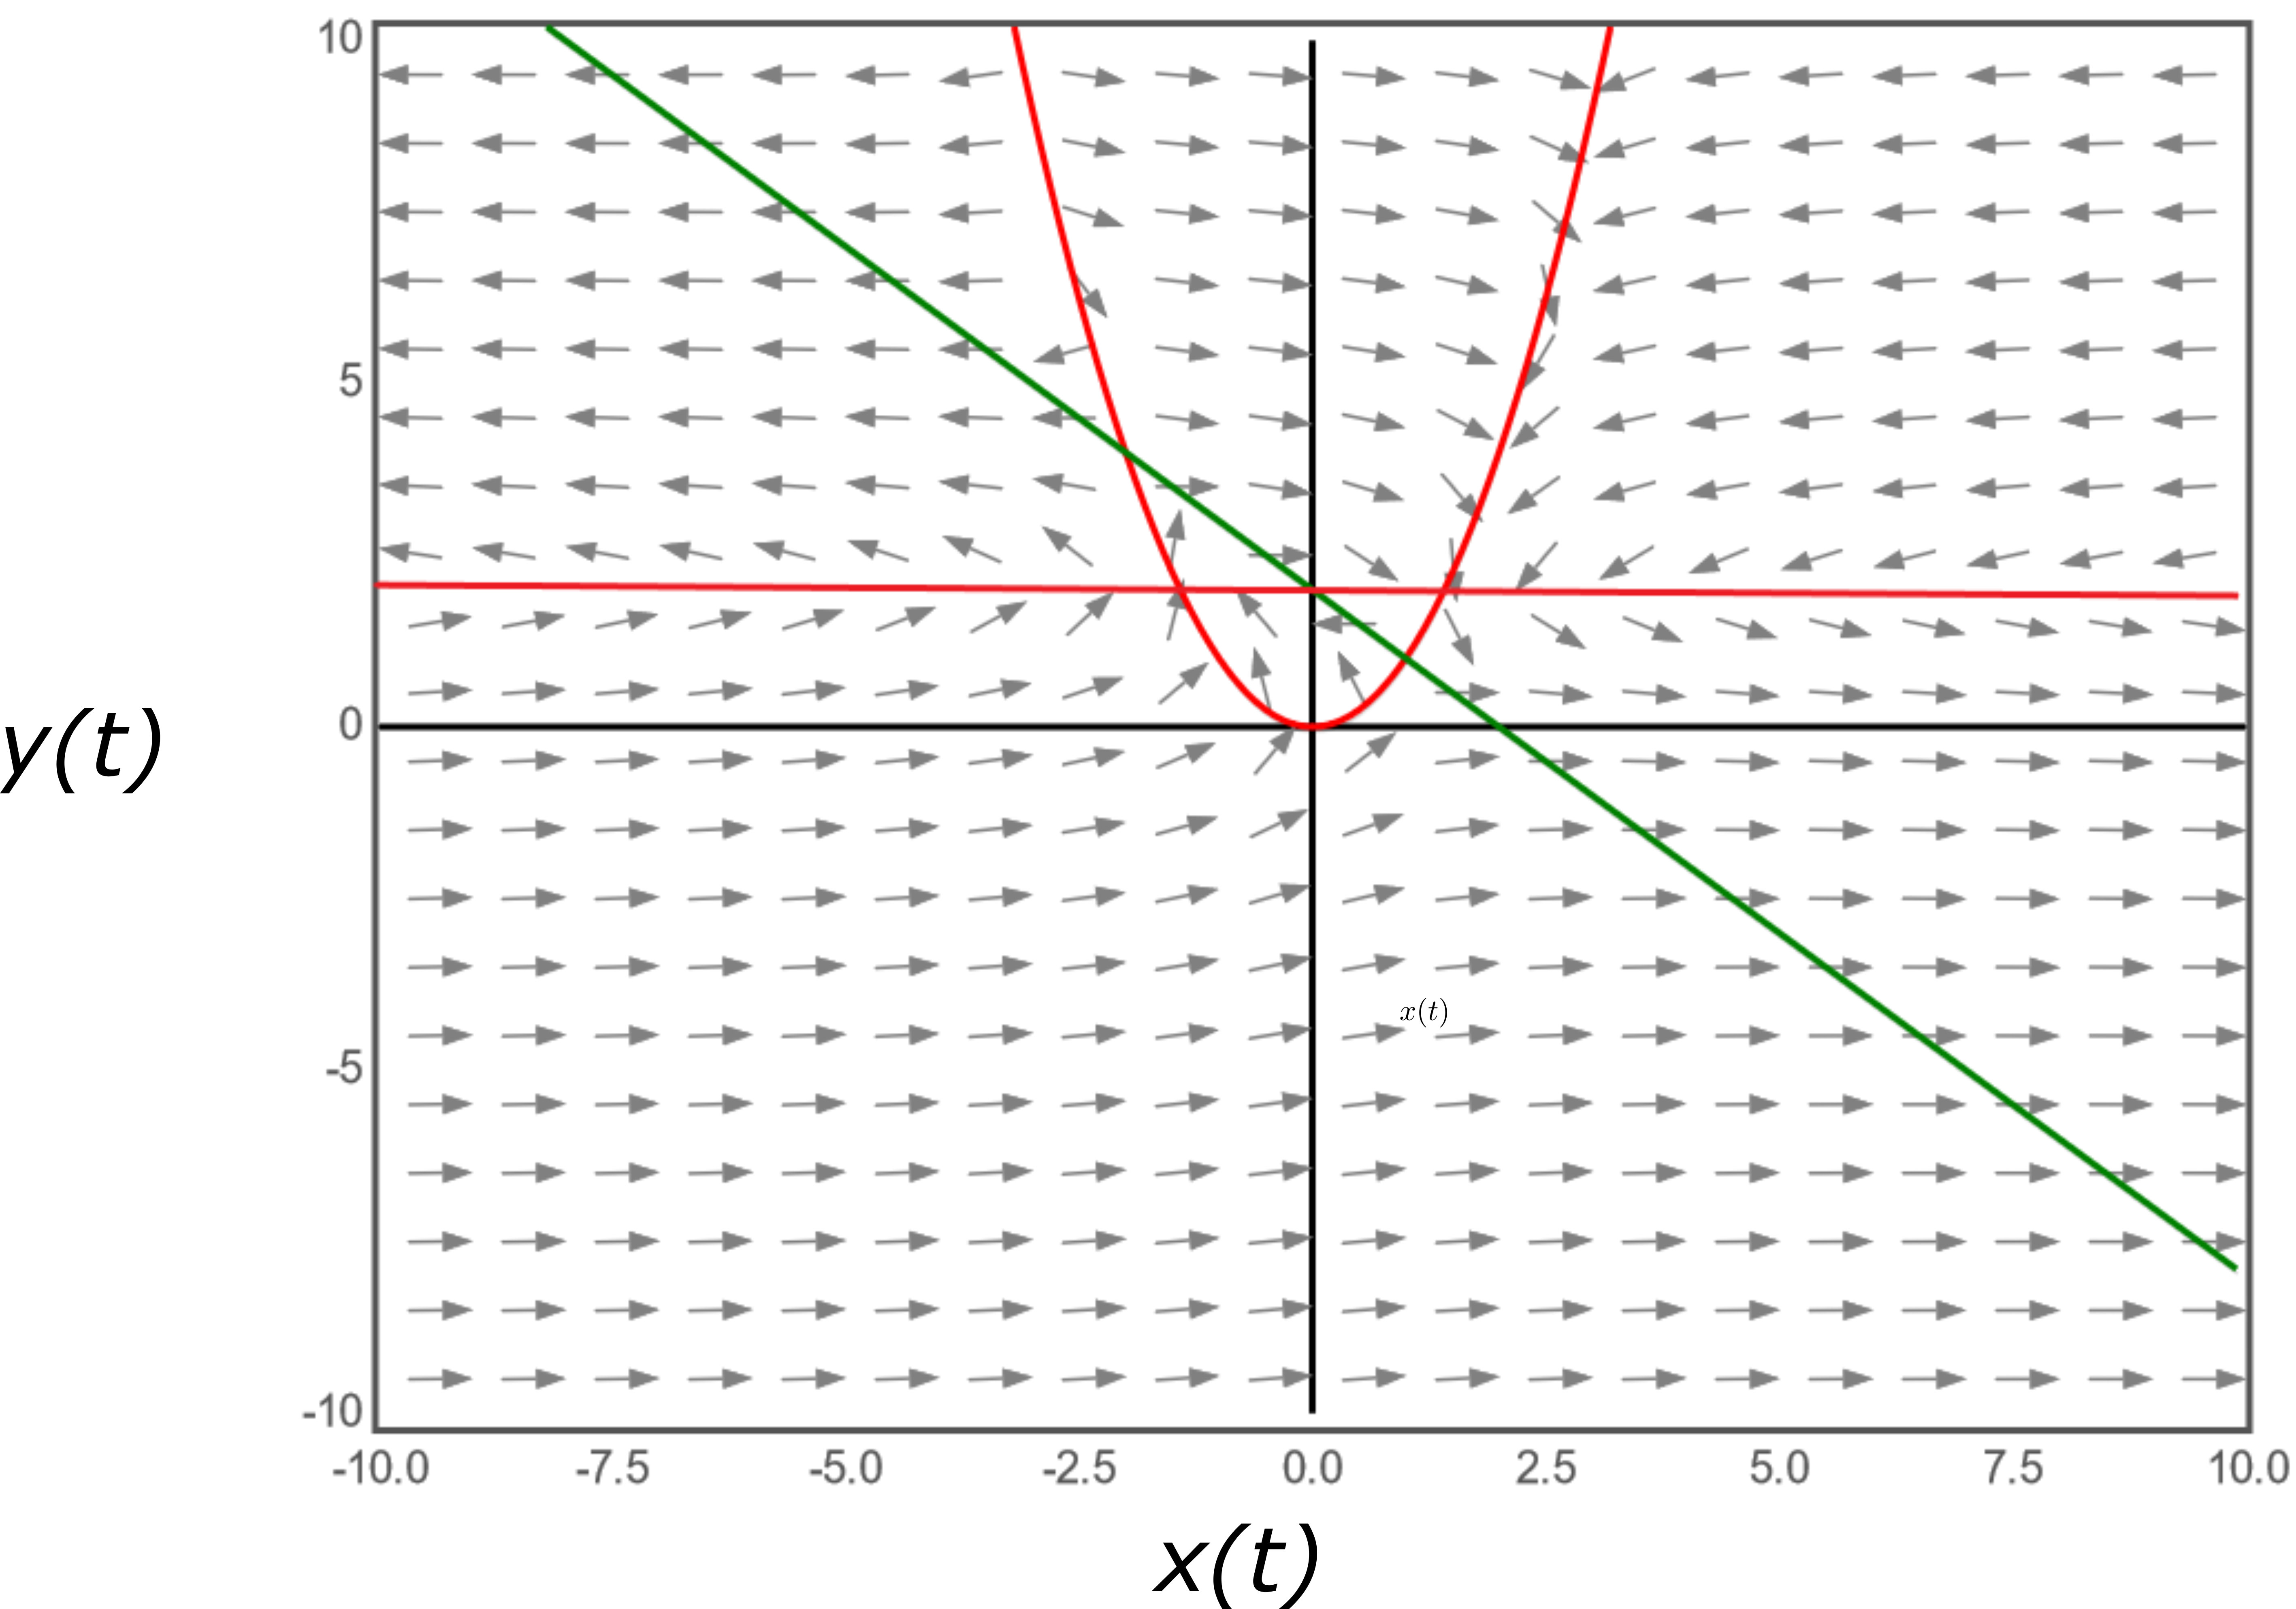
\includegraphics[scale=0.5]{media/image12.png}
                \end{center}

                To identify the critical points, we find the intersections of
                different nullclines. If $y = 2$, then $2 - x - 2 = 0
                \Longrightarrow x = 0$ so one critical point is $(0, 2)$. If $y
                = x^2$, then the equation for the $y$-nullcline becomes $2 - x -
                x^2 = 0 \Longrightarrow (2 + x)(1 - x) = 0 \Longrightarrow x =
                -2, x = 1$. Letting $x = -2$ yields the critical point $(-2,
                4)$ and letting $x = 1$ gives the critical point $(1, 1)$.

                The Jacobian matrix is given by
                \[
                J = 
                \begin{pmatrix}
                    \frac{\partial x'}{\partial x} & \frac{\partial x'}{\partial
                    y} \\
                    \frac{\partial y'}{\partial x} & \frac{\partial
                    y'}{\partial y}
                \end{pmatrix} =
                \begin{pmatrix}
                    4x - 2xy & 2y - x^2 - 2 \\
                    -1 & -1
                \end{pmatrix}
                \] 
                We can classify each critical point by evaluating the Jacobian
                at said points.
                \begin{gather*}
                    J(0, 2) = 
                    \begin{pmatrix}
                        0 & 2 \\
                        -1 & -1
                    \end{pmatrix} \Longrightarrow
                    (-\lambda)(-1 - \lambda) + 2 = \lambda^2 + \lambda
                    + 2 = 0 \\
                    \Longrightarrow \lambda = -\frac{1}{2} \pm
                    \frac{1}{2} \sqrt{-7}
                \end{gather*}
                Since the eigenvalues are complex with real part less than zero,
                the critical point $(0, 2)$ is a stable spiral.
                \begin{gather*}
                    J(-2, 4) =
                    \begin{pmatrix}
                        8 & 10 \\
                        -1 & -1
                    \end{pmatrix} \Longrightarrow
                    (8 - \lambda)(-1 - \lambda) + 10 = \lambda^2 - 7\lambda + 2 =
                    0 \\
                    \Longrightarrow \lambda = \frac{7}{2} \pm
                    \frac{1}{2}\sqrt{47}
                \end{gather*}
                Since both eigenvalues are real and greater than zero, the
                critical point $(-2, 4)$ is an unstable node.
                \begin{gather*}
                    J(1, 1) =
                    \begin{pmatrix}
                        2 & -1 \\
                        -1 & -1
                    \end{pmatrix} \Longrightarrow
                    (2-\lambda)(-1-\lambda) - 1 = \lambda^2 - \lambda - 3 = 0 \\
                    \Longrightarrow \lambda = \frac{1}{2} \pm \frac{1}{2}
                    \sqrt{13}
                \end{gather*}
                Since both eigenvalues are real with one being negative and the
                other being positive, the critical point $(1, 1)$ is an unstable
                saddle.
            \end{solution}

        \pagebreak

        % Problem 2
        \item (15 points) Use the Laplace transform to solve the following IVP.
            Please show your work.
            \[
                y'' + 3y' + 2y = u_4(t), \quad y(0) = 0, \quad y'(0)=\frac{1}{2}
            \] 

            \begin{solution}
                Taking the Laplace transform of both sides yields
                \[
                    s^2Y - sy(0) - y'(0) + 3(sY - y(0)) + 2Y = \frac{e^{-4s}}{s}
                \] 
                Plugging and rearranging, we obtain
                \[
                    Y(s^2 + 3s + 2) = \frac{e^{-4s}}{s} + \frac{1}{2}
                \] 
                or
                \[
                Y = \frac{e^{-4s}}{s^3 + 3s^2 + 2s} + \frac{1}{2s^2 + 6s + 4}.
                \] 
                We apply a shifting theorem to the left term, finding
                \[
                    L^{-1} \left\{ \frac{e^{-4s}}{s^3 + 3s^2 + 2s} \right\} = 
                    u_4(t) L^{-1} \left\{ \frac{1}{s^3 + 3s^2 + 2s} \right\}
                    (t-4)
                \] 
                We use partial fractions to find the above inverse Laplace
                transform, which gives
                \[
                    \frac{1}{s^3 + 3s^2 + 2s} = \frac{1}{s(s+1)(s+2)} =
                    \frac{1}{2s} - \frac{1}{s+1} + \frac{1}{2(s-2)}
                \] 
                Therefore,
                \[
                    L^{-1} \left\{ \frac{1}{s^3 + 3s^2 + 2s} \right\} =
                    \frac{1}{2} - e^{-t} + \frac{1}{2}e^{-2t}
                \] 
                Similarly, we use partial fractions to find the inverse Laplace
                transform of the term on the right.
                \[
                    \frac{1}{2s^2 + 6s + 4} = \frac{1}{2(s+1)(s+2)} =
                    \frac{1}{2(s+1)} - \frac{1}{2(s+2)}
                \] 
                so
                \[
                    L^{-1} \left\{ \frac{1}{2s^2 + 6s + 4} \right\} =
                    \frac{1}{2} (e^{-t} - e^{-2t})
                \] 
                Thus, we obtain a final answer of
                \[
                    y(t) = u_4(t) \left( \frac{1}{2} - e^{4 - t} +
                        \frac{1}{2}e^{8 - 2t}\right) + \frac{1}{2} \left( e^{-t}
                        - e^{-2t} \right)
                \] 
            \end{solution}

        \pagebreak

        % Problem 3
        \item (8 points) Use the Laplace transform to solve the following IVP.
            Please show your work.
            \[
                y'' + 2y' + 2y = \delta(t - \pi), \quad y(0) = 0, \quad y'(0)=1
            \] 

            \begin{solution}
                Taking the Laplace transform of both sides yields
                \[
                    s^2Y - sy(0) - y'(0) + 2(sY - y(0)) + 2Y = e^{-\pi s}
                \] 
                Rearranging, we get
                \[
                    Y(s^2 + 2s + 2) = e^{-\pi s} + 1
                \] 
                or
                \[
                Y = \frac{e^{-\pi s}}{s^2 + 2s + 2} + \frac{1}{s^2 + 2s + 2}.
                \] 
                We apply a shifting theorem to simplify the inverse Laplace
                transform of the left term.
                \begin{align*}
                    L^{-1} \left\{ \frac{e^{-\pi s}}{s^2 + 2s + 2} \right\} &=
                    u_\pi(t) L^{-1} \left\{ \frac{1}{s^2 + 2s + 2}
                    \right\} (t - \pi)
                \end{align*}
                Thus, we merely need to calculate the inverse Laplace transform
                above, which we do by completing the square.
                \begin{gather*}
                    L^{-1} \left\{ \frac{1}{s^2 + 2s + 2} \right\} = L^{-1}
                    \left\{ \frac{1}{(s + 1)^2 + 1} \right\} = e^{-t} 
                    \sin(t)
                \end{gather*}
                We have the solution
                \[
                    y(t) = u_\pi (t) e^{\pi - t} \sin(t - \pi) + e^{-t}\sin(t)
                \] 
            \end{solution}

        \pagebreak

        % Problem 4
        \item (10 points) Consider the following IVP.
            \[
                4y'' + 4y' + 17y = g(t), \quad y(0) = y'(0) = 0
            \] 
            \begin{enumerate}[label={(\alph*)}]
                \item Use the Laplace transform to determine an explicit
                    expression for $Y(s)$, which is the Laplace transform of
                    $y(t)$. You can leave your answer in terms of $G(s)$, which
                    is the Laplace transform of $g(t)$. Please show your work.
                \item Use your result from part (a), the convolution theorem,
                    and the inverse Laplace transform to obtain an explicit
                    expression for $y(t)$. Leave your answer in terms of a
                    convolution integral involving $g(t)$. Please show your
                    work.
            \end{enumerate}

            \begin{solution}
                We start by taking the Laplace transform of both sides, which
                gives
                \[
                    4(s^2Y - sy(0) - y'(0)) + 4(sY - y(0)) + 17Y = G(s)
                \] 
                Plugging in values and factoring yields
                \[
                    Y(s) (4s^2 + 4s + 17) = G(s)
                \] 
                or
                \[
                    Y = \frac{1}{4s^2 + 4s + 17} G(s).
                \] 
                By the convolution theorem, the right side is equal to the
                Laplace transform of the convolution of $f$ and $g$ where
                $L(f)$ is the left factor and $L(g) = G(s)$.
                We compute $f$ by taking the inverse Laplace transform of the
                left factor, obtaining
                \begin{align*}
                    f = L^{-1} \left\{ \frac{1}{4s^2 + 4s + 17} \right\} &=
                    \frac{1}{4} L^{-1} \left\{ \frac{1}{(s+\frac{1}{2})^2 + 4}
                        \right\} \\
                      &= \frac{1}{8} e^{-\frac{1}{2}t} \sin(2t)
                \end{align*}
                Then the convolution theorem implies that
                \[
                    y(t) = f * g = \int_{0}^{t} \frac{1}{8} e^{-\frac{1}{2}
                    \uptau} \sin(2 \uptau) g(t - \uptau) \, d\uptau
                \] 
            \end{solution}
    \end{enumerate}
\end{document}
